\documentclass[a0paper,%
               25pt,%
               margin=0mm,
               innermargin=15mm
               %titleinnersep=0mm%
               ]{de-tikzposter}  % See Section 3

%\documentclass[25pt,%
%			   a0paper,%
%			   portrait,%
%			   margin=20mm,%
%			   innermargin=15mm,%
%			   titleinnersep=8mm,%
%			   titletoblockverticalspace=20mm,%
%			   blocktitleinnersep=8mm,%
%			   blocktitlewidthratio=08,%
%			   blocktitlemaxwidth=25cm,%
%			   blockbodyinnersep=8mm,%
%			   blockverticalspace=15mm,%
%			   colspace=15mm,%
%			   subcolspace=8mm]{tikzposter}

\usepackage{natbib}
\usepackage{multicol}
%\usepackage[none]{hyphenat}
\usepackage[utf8]{inputenc}
\usepackage{de-authblk}
\usepackage{ngerman}
\usetheme{Basic}

%\usecolorstyle[colorPalette=Default]{Default}
\input mytikzpostercolourstyle.tex

%%%%%%%%%%%%%%%%%%%%%%%%%%%%%%%%%%%%%%%%%%%%%%%



\usebackgroundstyle{Empty} % oder {Empty}
\usetitlestyle{myTitle} % oder {Empty}
\useblockstyle{Basic} %oder {Default}
%\useinnerblockstyle{Table}

%\renewcommand\familydefault{cmss}
%\renewcommand\familydefault{helvetica}
%\usepackage{palatino}
\renewcommand{\familydefault}{\sfdefault}
%\fontfamily{ppl}\selectfont

\tikzposterlatexaffectionproofoff


\selectlanguage{ngerman}

\titlegraphic{~~~~~~~~~~~~~~~\includegraphics[scale=2.3]{fulogo}\hfill
\includegraphics[scale=2.8]{dfg_logo_blau_4c}\hfill
\includegraphics[scale=.7]{ids_logo_1c}~~~~
\includegraphics[height=3.8cm,width=8cm]{orange}}
\title{Induktive Topikmodellierung und extrinsische Topikdomänen} 
\author[1]{Felix Bildhauer}
\author[2]{Roland Schäfer}
\affil[1]{\Large Abteilung Grammatik, Institut für Deutsche Sprache, Mannheim}
\affil[2]{\Large Linguistische Webcharakterisierung (DFG), Freie Universität Berlin}

\makeatletter
\def\maketitle{\AB@maketitle}
\makeatother


%%%%%%%%%%%%%%%%%%%%%%%%%%%%%%%%%%



%%%%%%%%%%%%%%%%%%%%%%%%%%%%%%%%%%%%%%%%%%%%%%%%%%%%%%%%%%%%%%%%%%
%%%%%%%%%%%%%%%%%%%%%%%%%%%%%%%%%%%%%%%%%%%%%%%%%%%%%%%%%%%%%%%%%%



\begin{document}
\maketitle  % See Section 4.1
\raggedright

%\block{}{\centering \huge \textbf{Induzierte LSI-Topiks: Interpretation und Korpusvergleich}}

\begin{columns}
\column{.4}
\block{Induzierung von Topiks}{

\innerblock{Motivation}{

\begin{itemize}
  \item \raggedright Textklassifikation nach externen definierten Kategorien:\\subjektiv, viele unterschiedliche Taxonomien
  \item \raggedright Datengetriebenes Aufdecken von Topics: objektiver, aber Kategorien nicht immer interpretierbar und oft nicht wie von Linguisten erwünscht.
  \item \raggedright Vergleich von Korpora anhand induzierter Topiks
       (Korpusvergleich ist ein viel diskutiertes Thema: Kilgarriff 2001, Biemann et \textit{al.} 2013, Schäfer und Bildhauer 2013)
\end{itemize}
}

\innerblock{Korpora}{

%\begin{tabular}{ll}
%\textbf{870} Dokumente aus DECOW14 & (Schäfer und Bildhauer 2012)\\
%\textbf{886} Dokumente aus DeReKo 2014-II & (Kupietz et \textit{al}.\ 2010)\\
%\end{tabular}

\begin{itemize}
\item[] \textbf{870} Dokumente aus DECOW14 (Schäfer und Bildhauer 2012)
\item[] \textbf{886} Dokumente aus DeReKo 2014-II  (Kupietz et \textit{al}.\ 2010)
\end{itemize}
\vspace{.7cm}

\begin{itemize}
  \item DECOW14 (über 17 Mrd.\ Wörter) ist ein gecrawltes Webkorpus 
  \item DeReKo (über 28 Mrd.\ Wörter) enthält überwiegend Zeitungstexte
  \item Identische Aufbereitung aller Dokumente (Tokenisierung,\\PoS-Tagging, Lemmatisierung, Eigennamenerkennung).
\end{itemize}
}

\innerblock{Verfahren}{

\begin{itemize}
  \item \textit{Latent Semantic Indexing} (Landauer und Dumais 1994)\\
  %\cite{LandauerDumais1994}
   Implementierung aus \textit{Gensim} ({\v R}eh{\r u}{\v r}ek und Sojka 2010) 
  \item Beschränkung auf Substantive, Adjektive, Verben, Adverbien
  \item Lemma-PoS Paare (\texttt{haus\_nn}, \texttt{franzkafka\_ne} etc.)
\end{itemize}


}
\vspace{1.1cm}
}

\column{.6}
\block{LSI-Topiks: Interpretation und Korpusvergleich}{

\innerblock{Verhältnis relativer Häufigkeiten (log): Für jedes Korpus, Anteil der Dokumente,\\ für die LSI-Topik \textit{X} unter den drei am stärksten assozierten Topiks ist.}

 \begin{tikzfigure}%[Caption of the figure]
%     \label{fig:fig1}
%\includegraphics[scale=2.2]{testplot}     
 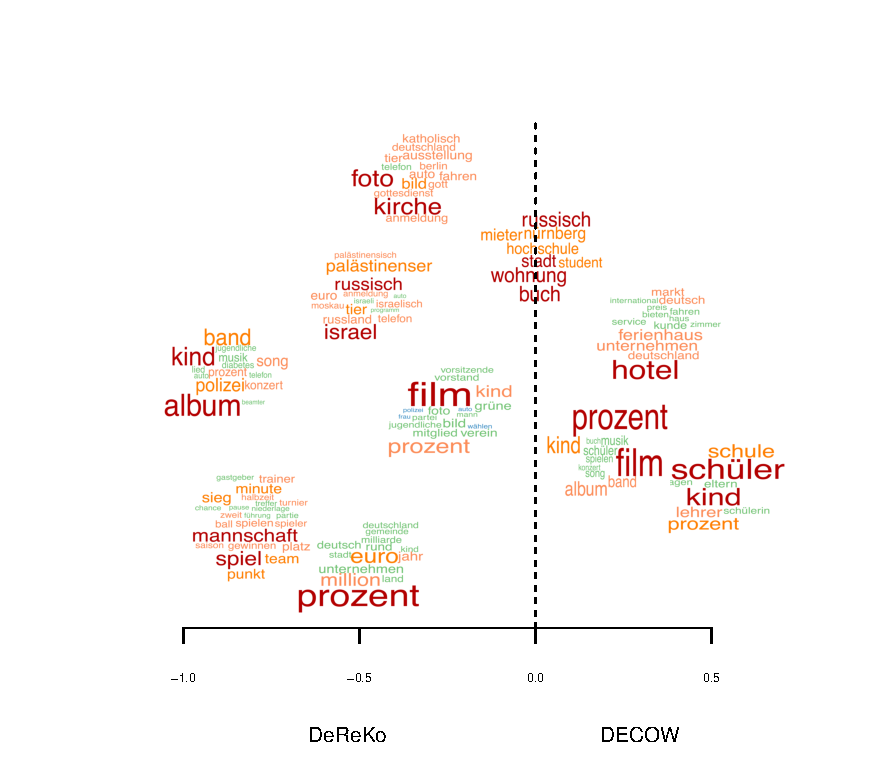
\includegraphics[scale=2.8]{topics-logratios2}
 \end{tikzfigure}


}
\end{columns}

%%%%%%%%%%%%%%%%%%%%%%%%%%%%%%%%%%%%%%%%%%%%%



\begin{columns}
\column{0.5}

\block{Topik-Domänen}{
\innerblock{Goldstandard-Daten}{Manuelle Annotation der DECOW- und DeReKo-Daten nach dem \textit{COWCat}-Schema:\\
 13 Kategorien für Topik-Domänen\\


\begin{tabular}{p{.12\textwidth}p{.12\textwidth}p{.12\textwidth}p{.12\textwidth}}
	\textit{Science} & \textit{Technology} &  \textit{Medical} & \textit{Fine-Arts}\\
	\textit{History} &  \textit{Business} & \textit{Law} &  \textit{Individuals}\\
	 \textit{Philosophy} & \textit{Beliefs} &   \textit{Life-and-Leisure} &\\
\textit{Public-Life-And-Infrastructure} & \textit{Politics-and-Society}
\end{tabular}
}


\begin{tikzfigure}[Verteilung der Dokumente auf Topik-Domänen in DECOW (links) und DeReKo (rechts)]
%     \label{fig:cow.cats}

\includegraphics[scale=1.2]{cow-cats2}~~~~~

\includegraphics[scale=1.2]{dereko-cats3}
 \end{tikzfigure}

}

\block{Maschinelles Lernen}{
Lassen sich Topik-Domänen aus den induzierten LSI-Topiks lernen?

\begin{itemize}
  \item Daten aus LSI mit unterschiedlichen Parametern 
  \begin{itemize}
  \item Vorverarbeitungsvarianten der Korpora
  \item Anzahl der Topiks (20--90)
  \item Menge zusätzlicher Dokumente für die Topikinduktion
\end{itemize}

  \item Klassifikator: SVM mit Pearson VII Kernel (Üstün et \textit{al.} 2006)
  \item Evaluation in verschiedenen Varianten:
\begin{itemize}
  \item Trainingsdaten vs.\ 10-fache Kreuzvalidierung
  \item voller Datensatz vs.\ reduzierter Datensatz (seltene Kategorien entfernt)
\end{itemize}

 
\end{itemize}

\vspace{1cm}
}

\column{0.5}
\block{Ergebnisse}{
\innerblock{Anteil korrekt klassifizierter Dokumente  für verschiedene \\Verarbeitungs- und Evaluierungsvarianten}


\begin{tikzfigure}[DECOW]
%     \label{fig:cow}
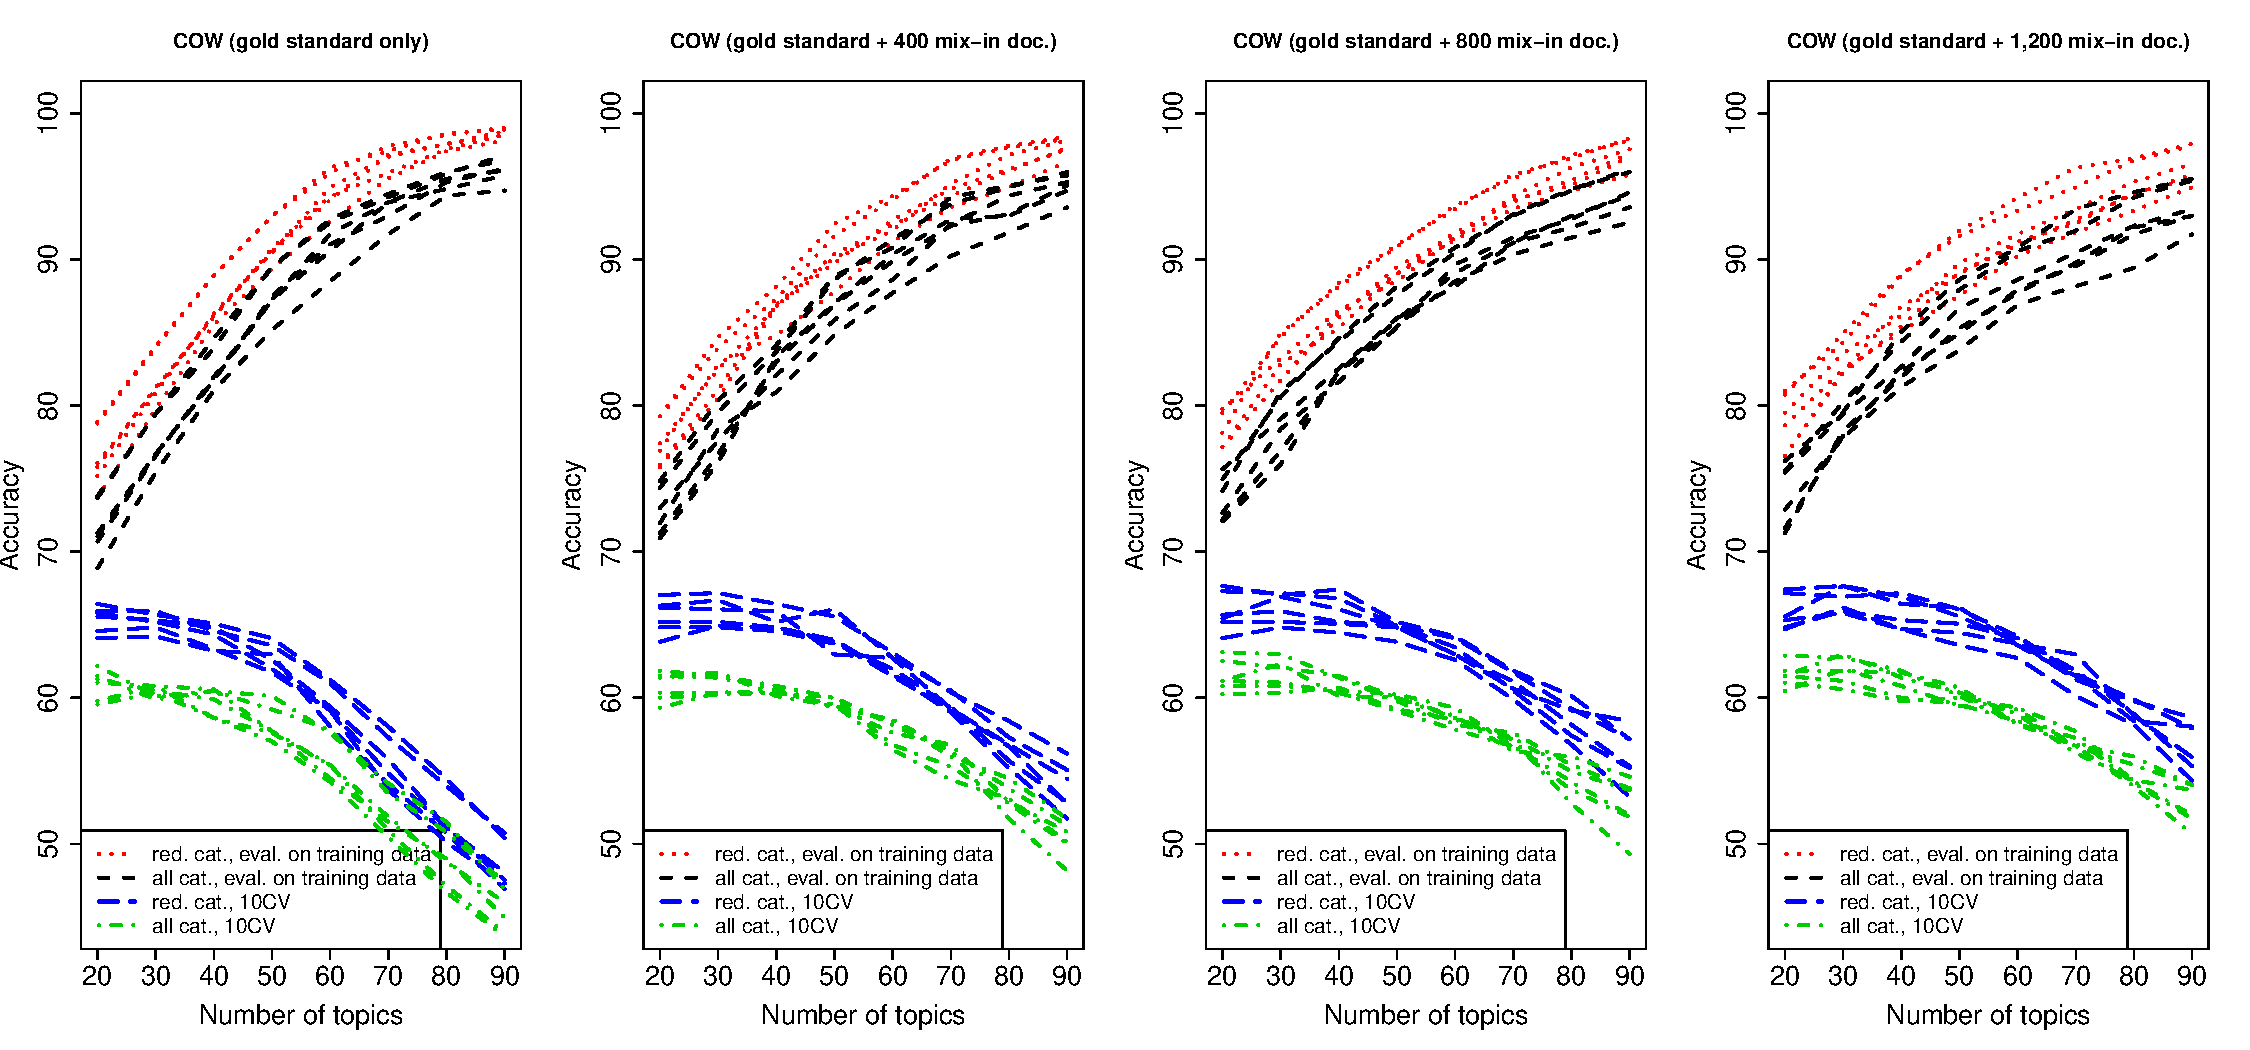
\includegraphics[scale=.6]{cow}
 \end{tikzfigure}

\begin{tikzfigure}[DeReKo]
%     \label{fig:dereko}
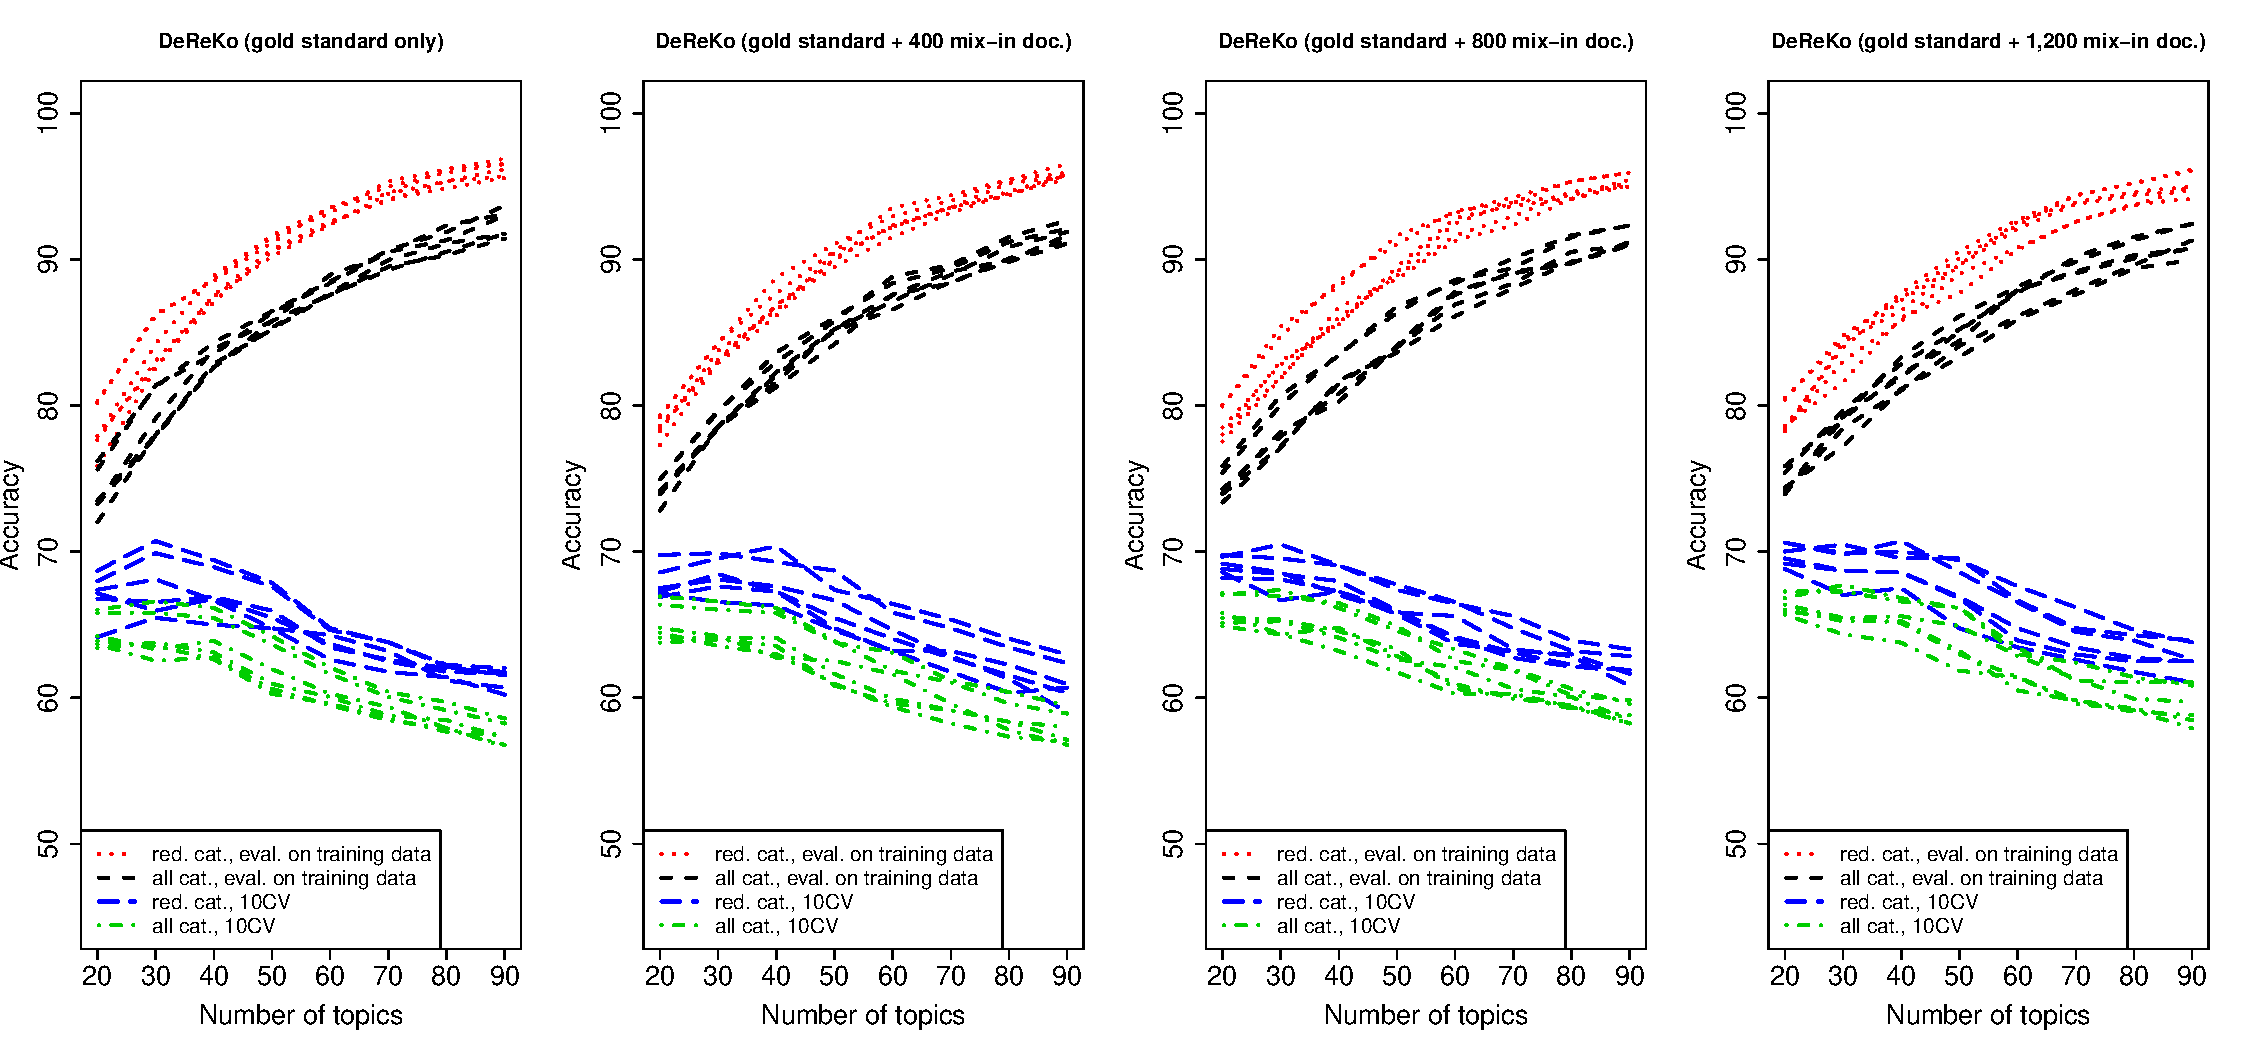
\includegraphics[scale=.6]{dereko} 
 \end{tikzfigure}
	

\begin{tikzfigure}[DECOW $\cup$ DeReKo]
%     \label{fig:coreko}
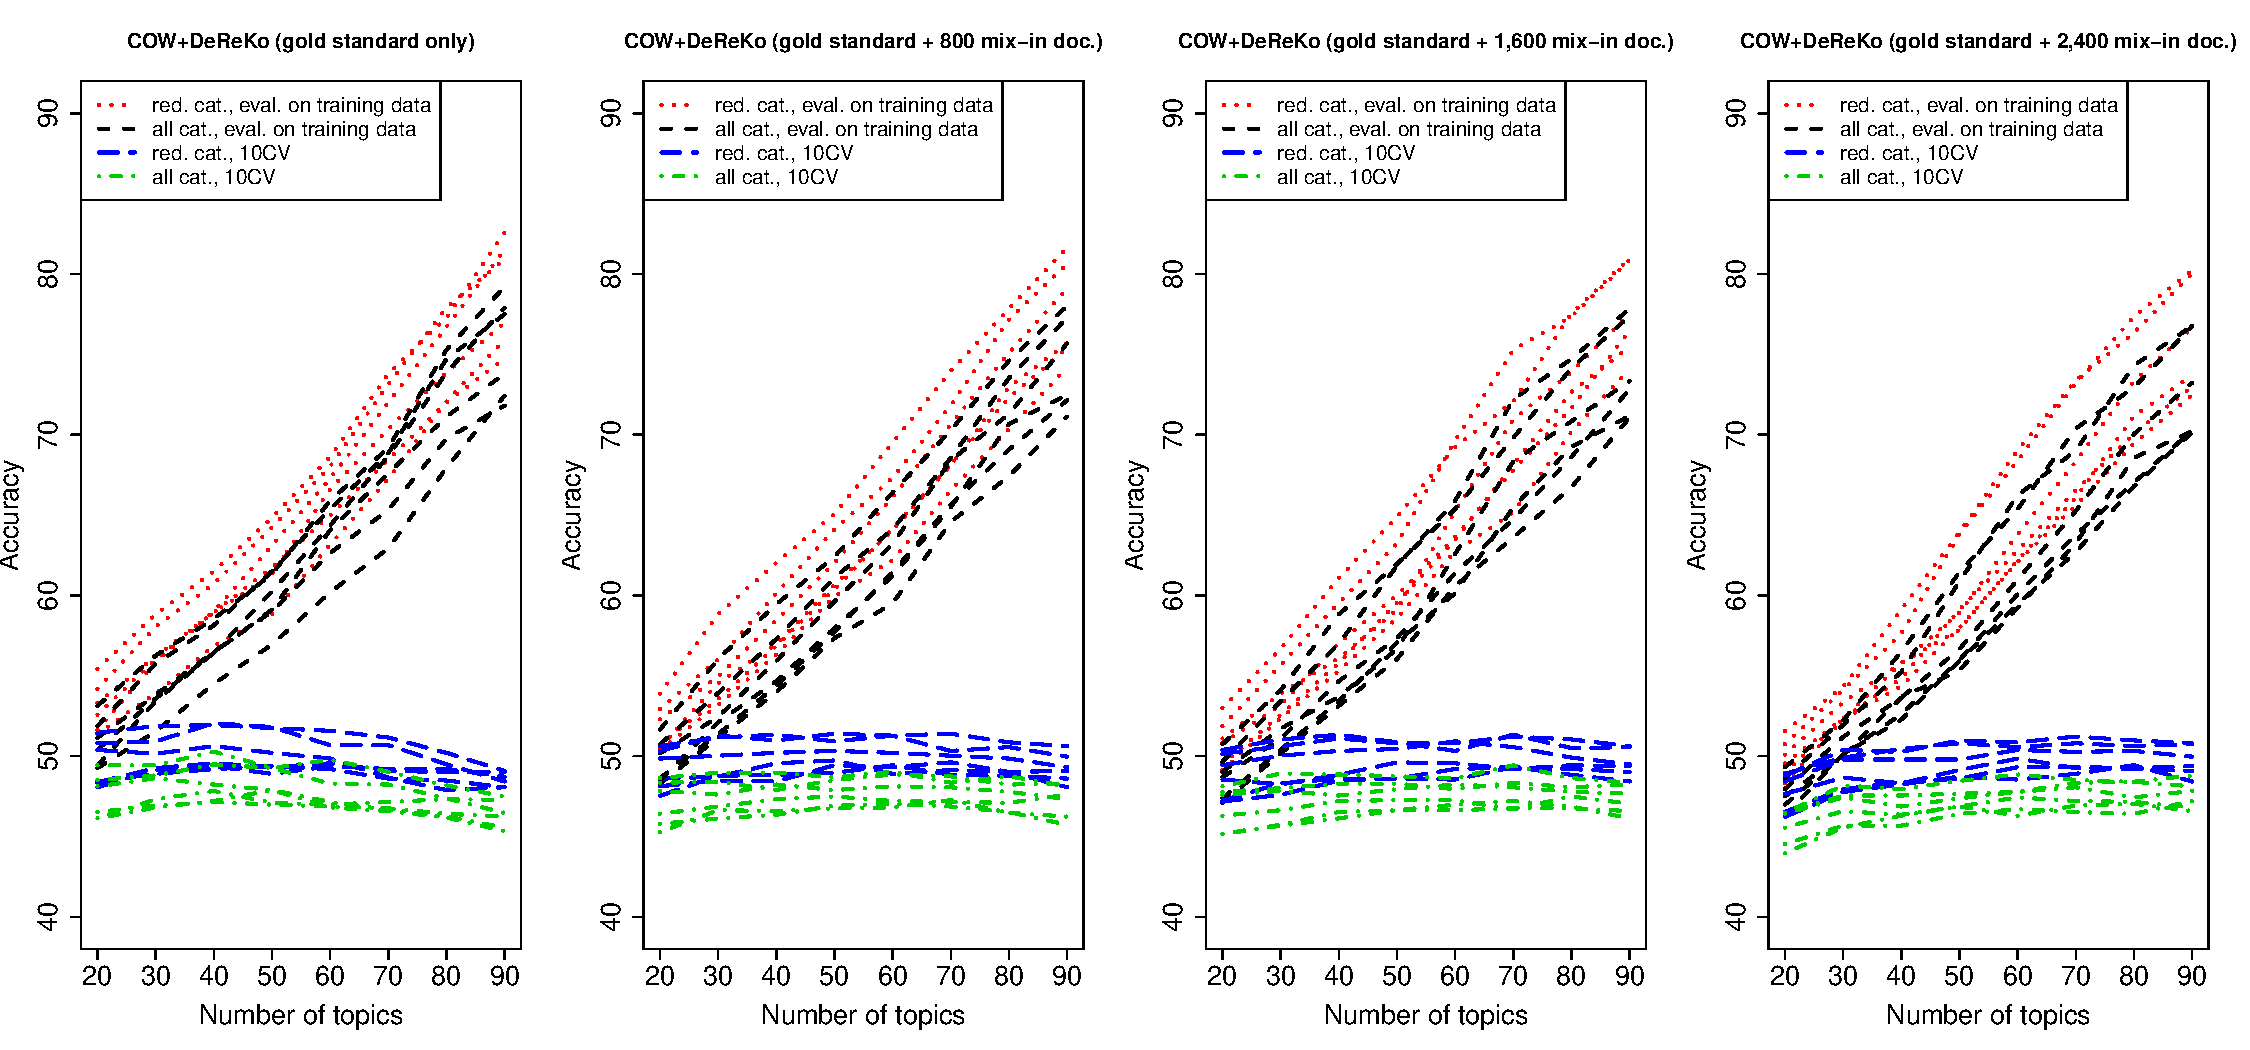
\includegraphics[scale=.6]{coreko}  
 \end{tikzfigure}	



%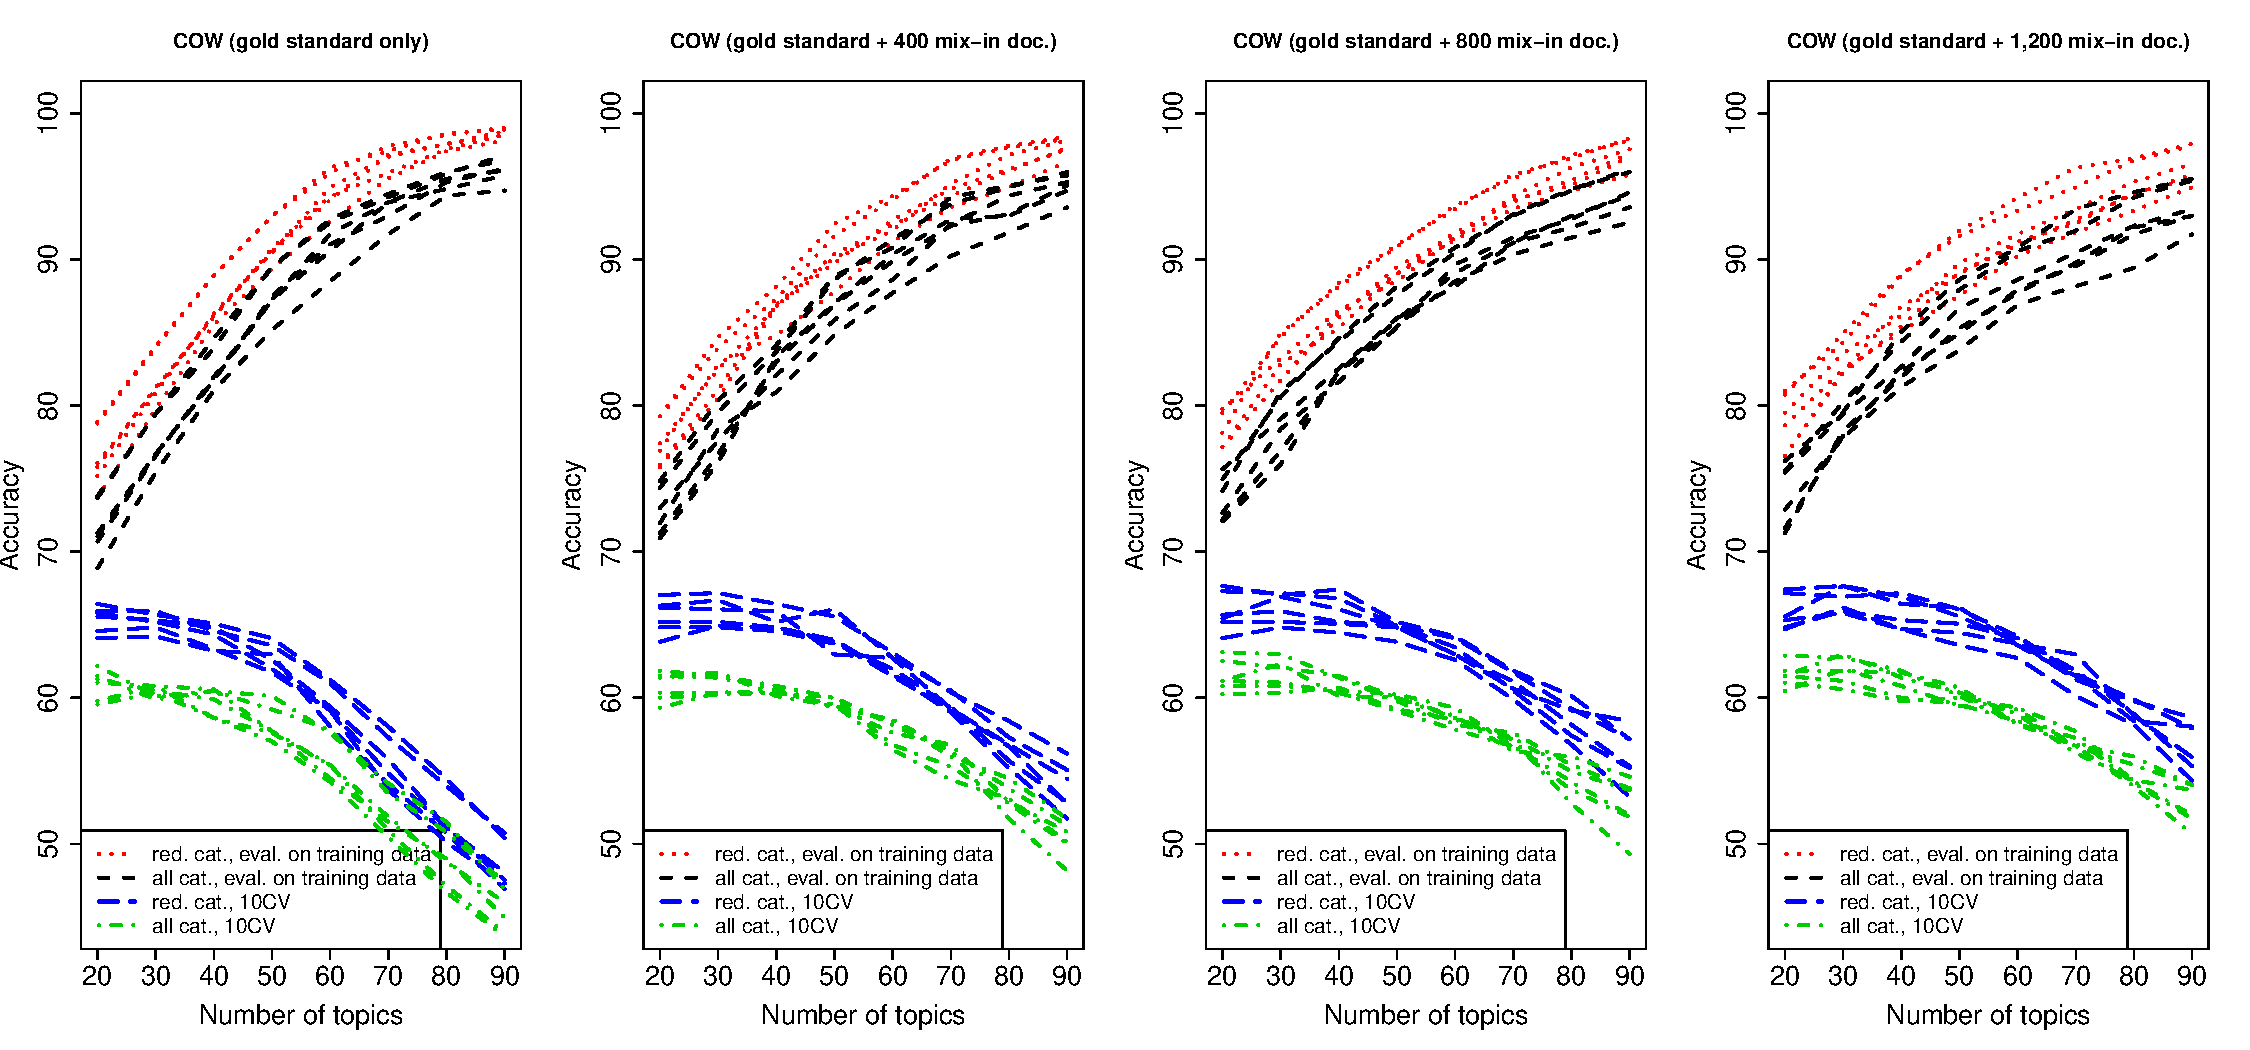
\includegraphics[scale=.7]{cow}  % See Section 4.2

%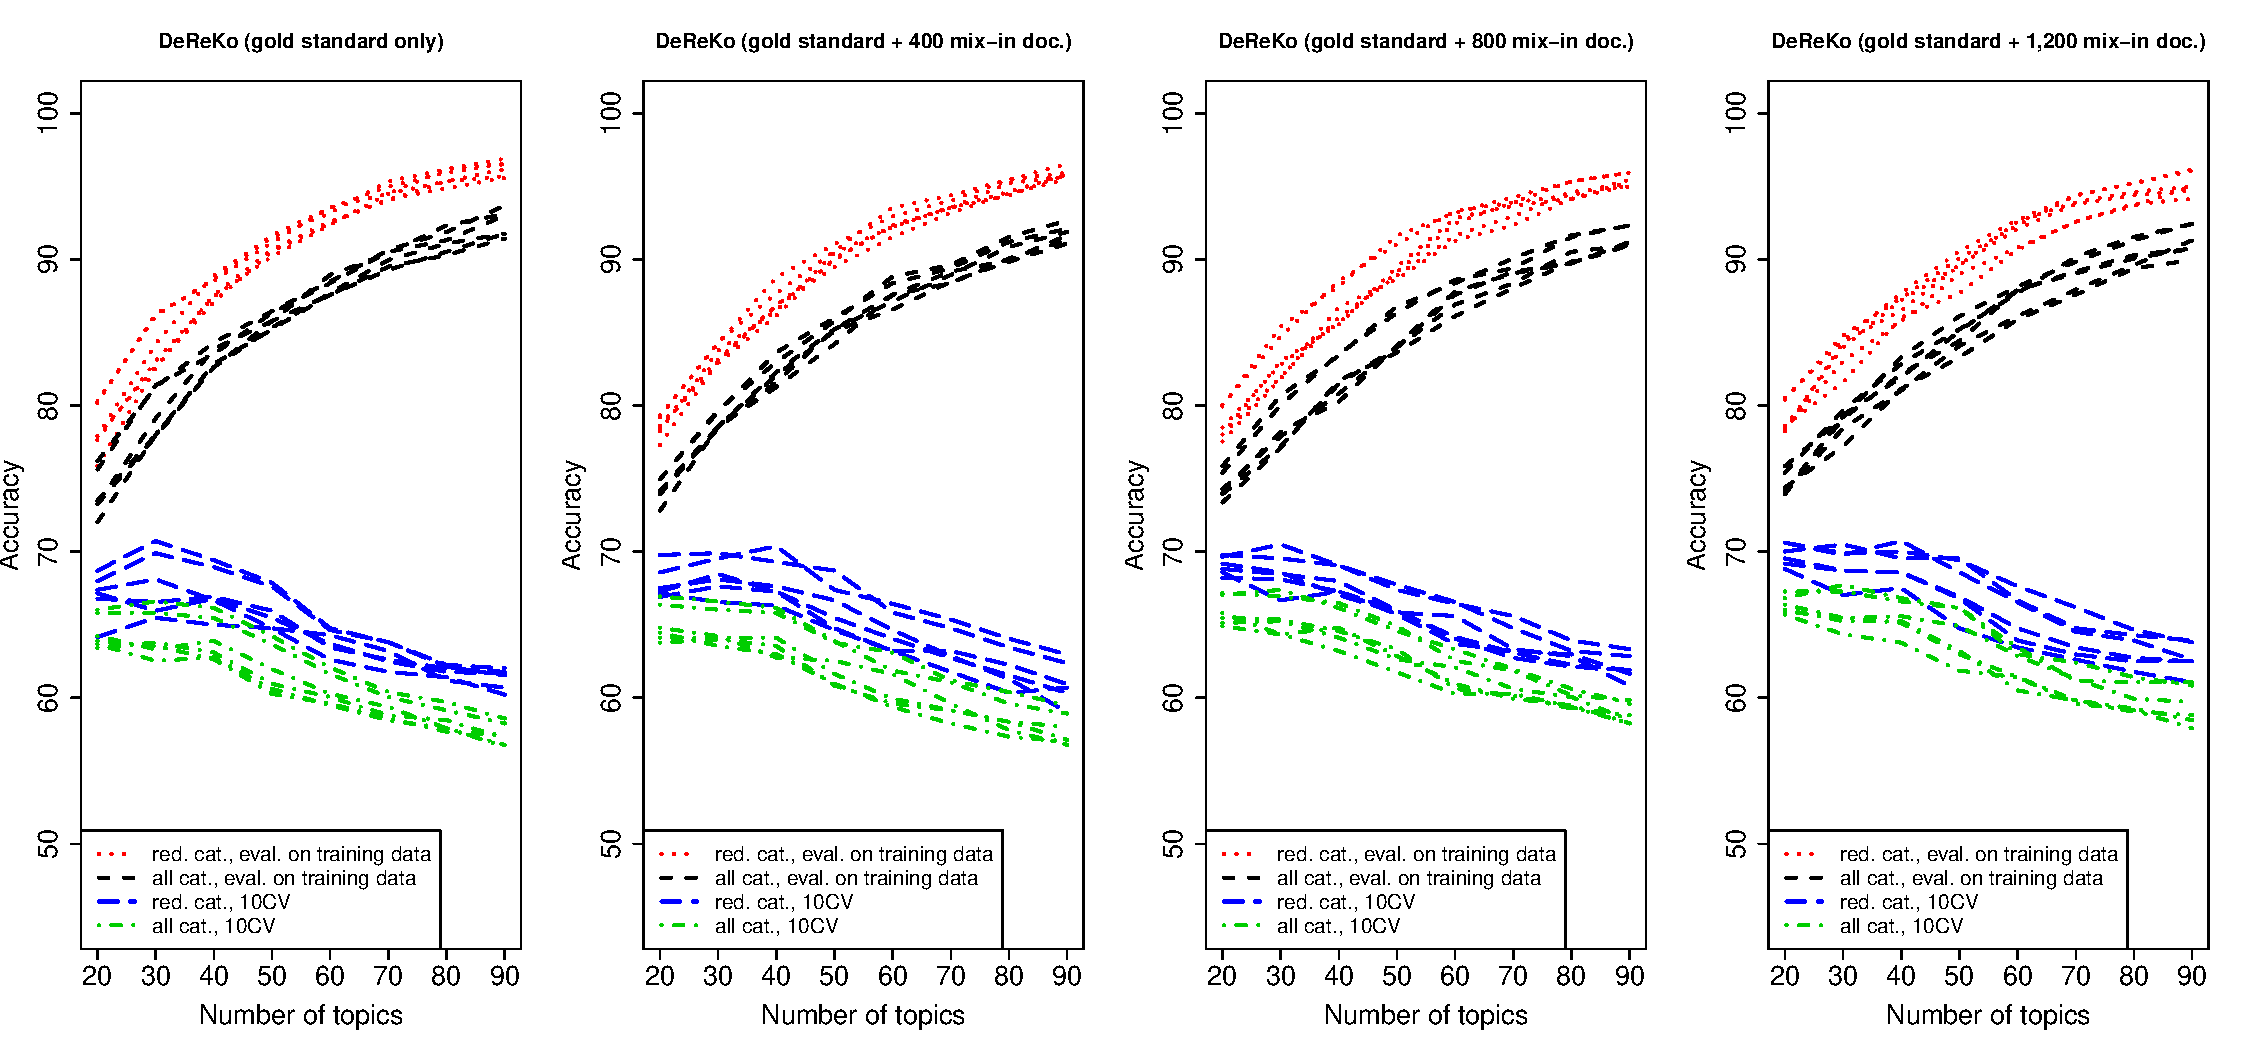
\includegraphics[scale=.7]{dereko}

%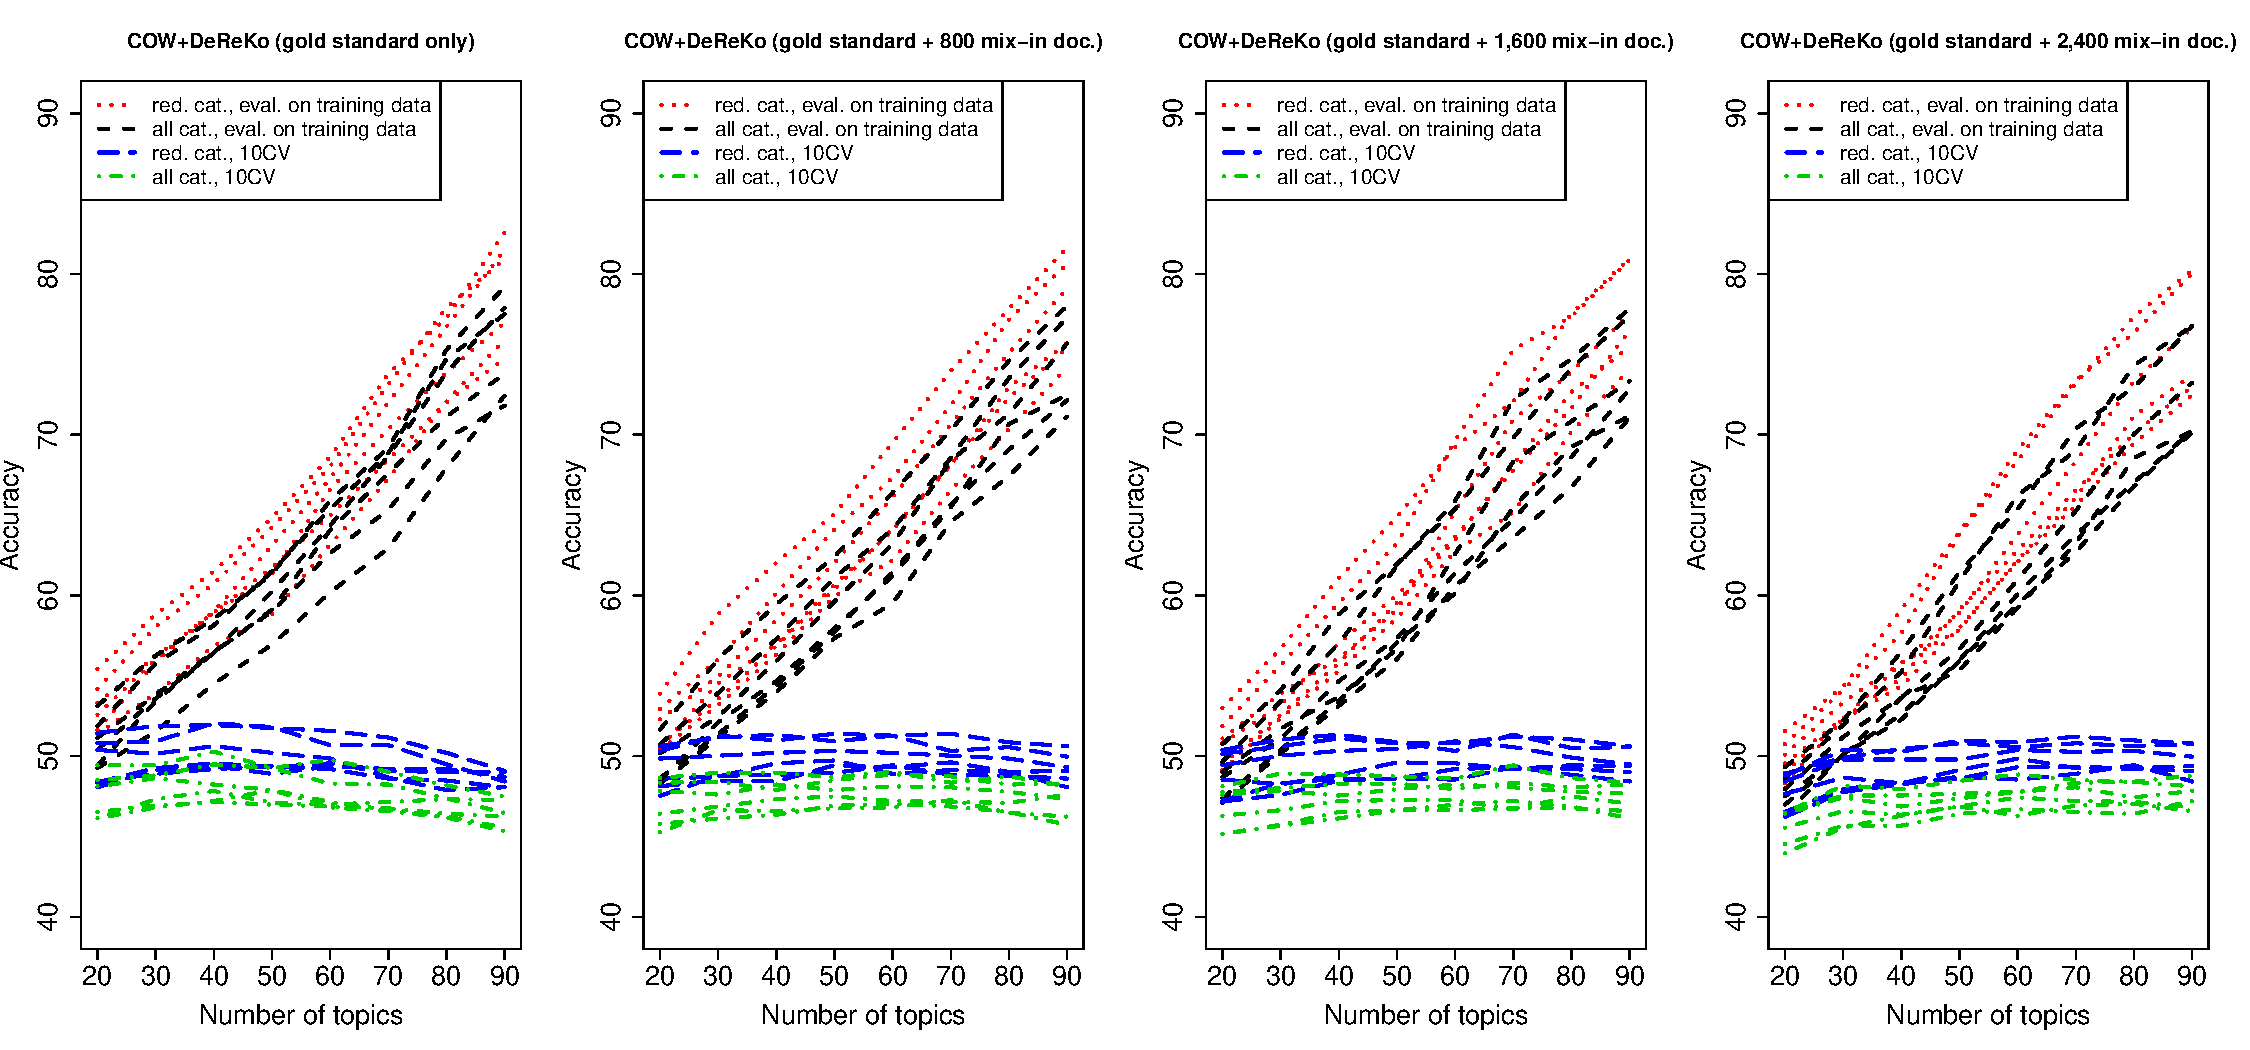
\includegraphics[scale=.7]{coreko}
}
%\end{minipage}

	%}
\end{columns}

%\block{}{
%\begin{multicols}{2}
%{\bibliography{BigBiblio}
%\bibliographystyle{natbib.myfullname}
%}
%\end{multicols}
%}

\end{document}
